\documentclass[preprint, 3p,
authoryear]{elsarticle} %review=doublespace preprint=single 5p=2 column
%%% Begin My package additions %%%%%%%%%%%%%%%%%%%

\usepackage[hyphens]{url}

  \journal{International Journal of Human-Computer
Studies} % Sets Journal name

\usepackage{lineno} % add

\usepackage{graphicx}
%%%%%%%%%%%%%%%% end my additions to header

\usepackage[T1]{fontenc}
\usepackage{lmodern}
\usepackage{amssymb,amsmath}
\usepackage{ifxetex,ifluatex}
\usepackage{fixltx2e} % provides \textsubscript
% use upquote if available, for straight quotes in verbatim environments
\IfFileExists{upquote.sty}{\usepackage{upquote}}{}
\ifnum 0\ifxetex 1\fi\ifluatex 1\fi=0 % if pdftex
  \usepackage[utf8]{inputenc}
\else % if luatex or xelatex
  \usepackage{fontspec}
  \ifxetex
    \usepackage{xltxtra,xunicode}
  \fi
  \defaultfontfeatures{Mapping=tex-text,Scale=MatchLowercase}
  \newcommand{\euro}{€}
\fi
% use microtype if available
\IfFileExists{microtype.sty}{\usepackage{microtype}}{}
\usepackage[]{natbib}
\bibliographystyle{plainnat}

\ifxetex
  \usepackage[setpagesize=false, % page size defined by xetex
              unicode=false, % unicode breaks when used with xetex
              xetex]{hyperref}
\else
  \usepackage[unicode=true]{hyperref}
\fi
\hypersetup{breaklinks=true,
            bookmarks=true,
            pdfauthor={},
            pdftitle={The Effects of Contrast on Correlation Perception in Scatterplots},
            colorlinks=false,
            urlcolor=blue,
            linkcolor=magenta,
            pdfborder={0 0 0}}

\setcounter{secnumdepth}{5}
% Pandoc toggle for numbering sections (defaults to be off)


% tightlist command for lists without linebreak
\providecommand{\tightlist}{%
  \setlength{\itemsep}{0pt}\setlength{\parskip}{0pt}}



\usepackage{booktabs}
\usepackage{longtable}
\usepackage{array}
\usepackage{multirow}
\usepackage{wrapfig}
\usepackage{float}
\usepackage{colortbl}
\usepackage{pdflscape}
\usepackage{tabu}
\usepackage{threeparttable}
\usepackage{threeparttablex}
\usepackage[normalem]{ulem}
\usepackage{makecell}
\usepackage{xcolor}



\begin{document}


\begin{frontmatter}

  \title{The Effects of Contrast on Correlation Perception in
Scatterplots}
    \author[CS]{Gabriel Strain%
  \corref{cor1}%
  }
   \ead{Gabriel.Strain@manchester.ac.uk} 
    \author[CS]{Andrew J. Stewart%
  %
  }
   \ead{Andrew.J.Stewart@manchester.ac.uk} 
    \author[SSS]{Paul Warren%
  %
  }
   \ead{Paul.Warren@manchester.ac.uk} 
    \author[CS]{Caroline Jay%
  %
  }
   \ead{Caroline.Jay@manchester.ac.uk} 
      \affiliation[CS]{Department of Computer Science, Faculty of
Science and Engineering, University of Manchester, Oxford Road,
Manchester, M13 9PL, United Kingdom.}
    \affiliation[SSS]{Division of Psychology, Communication and Human
Neuroscience, School of Health Sciences, Faculty of Biology, Medicine,
and Health, University of Manchester, Oxford Road, Manchester, M13 9PL,
United Kingdom.}
    \cortext[cor1]{Corresponding author}
  
  \begin{abstract}
  Scatterplots are common data visualizations that can be used to
  communicate a range of ideas, primarily the correlation between two
  variables. Despite their ubiquity, people typically do not perceive
  correlations between variables accurately from scatterplots, tending
  to underestimate the strength of the relationship displayed. Here we
  describe a two-experiment study in which we adjust the visual contrast
  of scatterplot points, and demonstrate a systematic approach to
  altering the bias. We find evidence that lowering the total visual
  contrast in a plot leads to increased bias in correlation estimates
  and show that decreasing the salience of points as a function of their
  distance from the regression line, by lowering their contrast, can
  facilitate more accurate correlation perception. We discuss the
  implications of these findings for visualization design, and provide a
  framework for online, reproducible, and large-sample-size (N = 150 per
  experiment) testing of the design parameters of data visualizations.
  \end{abstract}
    \begin{keyword}
    Scatterplot \sep Correlation Perception \sep Crowdsourced \sep 
    Data visualization
  \end{keyword}
  
 \end{frontmatter}

\hypertarget{introduction}{%
\section{Introduction}\label{introduction}}

In one form or another, data visualizations have been used for thousands
of years to aid analysis, to supplement narrative prose, and to
communicate ideas \citep{azzam_2013}. Where once they were the preserve
of those working directly with data, it is now expected that most
professionals, and indeed many members of the public, are comfortable
and familiar with an array of different data visualizations. The
widespread adoption of data visualizations is positive for science as
effective data visualizations can aid communication, but it also brings
with it obligations, not only to design and communicate with honesty,
but also to study how people understand and work with data
visualizations.

In the last two centuries, the use of data visualizations has become
increasingly common \citep{friendly_2005, azzam_2013}. The speed of the
adoption of visualizations has meant rigorous scientific study of how
they are comprehended by a viewer has often failed to keep pace. For
many people, the COVID-19 pandemic has made data visualizations an
everyday phenomenon (see \citet{bbc_2022} for examples of the types of
visualizations many saw daily). As data visualization designers, we have
a duty to design in such a way that viewers with little to no formal
statistical or data training can understand the message that
visualizations are trying to convey.

In this paper we present a novel visualization technique that
significantly increases the accuracy of people's performance on
correlation estimation tasks. In our first experiment, we show that
manipulating the contrast of scatterplot points can bias participants'
estimates of correlation. In our second we leverage this effect to
partially correct for a systematic underestimation by viewers of
correlations in scatterplots that has a long-standing basis in the
literature. Through this work we also present a framework for the
effective, inexpensive, and high-powered study of data visualizations.

\hypertarget{why-study-scatterplots}{%
\subsection{Why Study Scatterplots?}\label{why-study-scatterplots}}

Scatterplots, estimated in 1983 to account for between 70 and 80 percent
of data visualizations in scientific publications \citep{tufte_1983},
are simple representations of bivariate data that people generally
interpret in the same way \citep{kay_heer_2015}. \citet{rensink_2014}
identifies them as similar to a fruit fly for geneticists; simple enough
to be easily studied, but complex enough to provide interesting
insights. These features make them ideal candidates for controlled,
empirical study, in addition to providing us with insights into
visualization design and perception.

\hypertarget{related-work}{%
\section{Related Work}\label{related-work}}

\hypertarget{testing}{%
\subsection{Testing Correlation Perception}\label{testing}}

The primary concept communicated by scatterplots is correlation, (i.e
the strength of the relationship between two variables). Throughout this
paper we refer to an \emph{r} value, or the Pearson product moment
correlation coefficient. Pearson's \emph{r} takes a value between 0 and
\textbar1\textbar, and is positive or negative depending on the
direction of the relationship between the two variables in question.

Scatterplots have been extensively studied in a variety of experimental
paradigms. Very early work \citep{pollack_1960} asked participants to
make discriminative judgements between scatterplots with different
correlations, and found that people were more easily able to
discriminate as the magnitude of the \emph{r} value increased.
Subsequent work focused on asking participants to provide a numerical
estimate of the \emph{r} value, with studies finding evidence for a
systematic underestimation for positive \emph{r} values apart from 0 and
1. In several studies this effect was particularly pronounced for 0.2
\textless{} \emph{r} \textless{} 0.6
\citep{strahan_1978, bobko_1979, cleveland_1982, lane_1985, lauer_1989, collyer_1990, meyer_1992},
see Figure \ref{underestimation-curve} for an approximation of the
underestimation observed. In addition to studies employing
discriminative judgement or direct estimation tasks, several more recent
investigations have employed a combination of bisection tasks, in which
participants are asked to adjust a test plot so that its correlation is
halfway between two reference plots, and a staircase discriminative
judgement task that allows researchers to find the
just-noticeable-difference (JND) between scatterplots such that their
correlations are distinguishable 75\% of the time. This novel approach
\citep{rensink_2010} allows researchers to obtain measurements for
participants' precision and accuracy in correlation estimation, and to
begin to fit mathematical models that describe the relationship between
objective and perceived correlation. Given that this paper seeks to
provide design guidelines, and is interested in comparative,
naturalistic judgements of correlation, we have elected to use a direct
estimation paradigm.

\begin{figure}

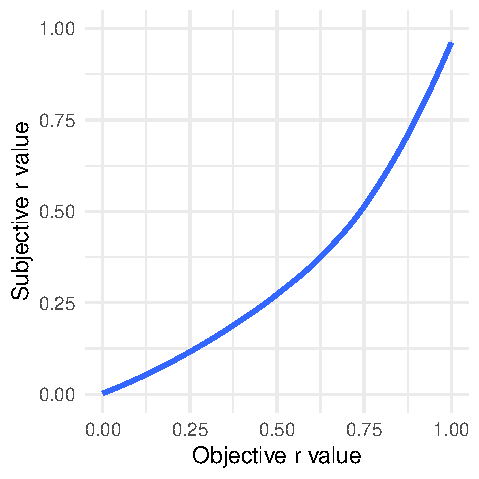
\includegraphics{contrast_and_scatterplots_files/figure-latex/underestimation-curve-1} \hfill{}

\caption{\label{underestimation-curve}Using a function that relates objective to subjective \textit{r} supplied in \cite{rensink_2017} allows us to visualize the nature of the underestimation curve found in correlation perception studies. The curve represents the underestimation of correlation.}\label{fig:underestimation-curve}
\end{figure}

\hypertarget{what-drives-correlation-perception}{%
\subsection{What Drives Correlation
Perception?}\label{what-drives-correlation-perception}}

Several key pieces of evidence point to correlation perception being
driven by the shape of the probability distribution relayed by the
points. A study investigating the effect of increasing the x and y
scales on scatterplots (thereby decreasing the size of the point cloud)
\citep{cleveland_1982} found that a viewer's judged association
increased as the size of the point cloud decreased, despite the \emph{r}
value remaining the same between conditions. The authors suggest this
may be due to participants using the area of the point cloud, or the
ratio of the minor and major axes of it, to judge association.
Decreasing the size of the point cloud here has also had the effect of
narrowing the width of the distribution displayed, as the length of the
minor axis has decreased.

Furthermore, another study asked participants to provide estimates of
correlation in scatterplots \citep{meyer_1997}. It found that the
relationship between objective and perceived \emph{r} values could be
accurately described by a function that included the mean of the
geometrical distances between the points and the regression line. This
is intuitive, as scatterplots with higher correlation will generally
have lower distances between their points and the regression line.

A more recent study investigating the hypothesis that people use visual
features to judge correlation \citep{yang_2019} found evidence that
several visual features were predictive of correlation estimation
performance. Among these was the standard deviation of all perpendicular
distances from the points to the regression line, a quantity similar to
that in \citet{meyer_1997}, which on an individual level was more
predictive of participants' estimates of correlation than the objective
\emph{r} value itself.

Bringing together work that has sought to model the relationship between
objective and perceived \emph{r} values, \citet{rensink_2017} notes that
equations for both discrimination and magnitude estimation include a
parameter, termed \emph{u} in \citet{rensink_2017}, that is small when
\emph{r} = 1, and increases as \emph{r} approaches 0. The utility of
this parameter in modelling correlation perception is indifferent to the
type of data visualization used, which implies that the width of the
probability distribution, summarised by the aforementioned parameter, is
key to how people estimate correlation. Within the context of
scatterplots however, this parameter can also be expressed as the
average distance between the points and the regression line (the
\emph{X} parameter in \citep{meyer_1997}).

None of the above is proof that people are using \emph{only} the mean or
standard deviation of geometrical distances between the points and the
regression line to estimate correlation. However, taken with findings
that correlation is perceived rapidly by viewers \citep{rensink_2014},
what we have discussed thus far suggests that this parameter is at least
a good proxy for what people are really attending to, insofar as
changing it has the ability to influence how people estimate
correlation. From this evidence, a good candidate for influencing
people's perceptions of correlation is changing the perceived width of
this probability distribution by changing the perceived distance between
points and the regression line.

\hypertarget{contrast}{%
\subsection{Contrast}\label{contrast}}

Adjusting the contrast in scatterplots has been used extensively to
solve problems of overplotting \citep{matejka_2015, bertini_2004}, in
which scatterplots with very large numbers of data points suffer from
visibility issues caused by excessive point density. Lowering the
contrast of all points makes the underlying distributions and trends
much easier to discern for the user. Despite the popularity of this
technique, little investigation has taken place into the effects of
reducing point contrast on people's perceptions of correlation; what has
been found is that correlation perception seems to be invariant to
changes in point contrast \citep{rensink_2012}, although this work took
place with small sample sizes (n = 12), and using only bisection/JND
methodologies.

Changing the contrast of a visual stimulus effectively reduces the
strength of that signal. A likely consequence of this is increased
uncertainty in aspects of that stimulus, for example the locations of
points in scatterplots. Consequently, one might anticipate that
increased noise could lead to altered perception of correlation and/or
more noise in correlation estimates due to effects on the perceived
position of points within the cloud. While there is indeed evidence
\citep{wehrhahn_1990} that the perception of stimulus position becomes
exponentially worse as contrast is reduced (as measured by vernier
acuity tasks), this is only true for a narrow range of low contrasts
just above the detection threshold. For higher contrasts vernier acuity
appears largely robust to such changes. Nonetheless, there is clear
evidence that other perceptual estimates become more uncertain with
reduced contrast, for example speed perception in \citet{champion_2017}.
With this in mind, and the relatively small sample size used in
\citet{rensink_2012}, we suggest that the effects of contrast on
perceived correlation warrant further investigation.

A recent study \citep{hong_2021} used contrast and size to encode a
third variable in trivariate scatterplots. The authors then asked
participants to use a mouse to click on the average position of all the
points displayed. They found that participants' estimates of average
point position were biased towards larger or darker points, which the
authors term the \emph{weighted average illusion}. Together with
evidence that darker and larger points are more salient
\citep{healey_2012}, this implies that we can use contrast to reduce the
salience of the points representing the widest parts of the probability
distribution; if this is successful, and participants perceive a
narrower distribution, we would expect this to be able to correct for a
viewer's underestimation bias.

One way to correct for an underestimation in correlation would be to
simply remove outer data points until correlation perception is aligned
with the actual correlation value. However, this would necessitate
hiding data, thus changing the information presented to the viewer. An
alternative approach is to manipulate the contrast of only some of the
points; it would seem most sensible to do so for the points that are
more extreme relative to the underlying regression line.

In the present study we address the issues raised above in two online
experiments with large sample sizes. In the first we consider the
effects of point contrast over the entire scatterplot on correlation
estimates. In the second experiment we examine how changing contrast as
a function of distance to the regression line affects perceived
correlation. To pre-empt our results we find clear effects of both
manipulations.

\hypertarget{general-methods}{%
\section{General Methods}\label{general-methods}}

\hypertarget{formalising-contrast}{%
\subsection{Formalising Contrast}\label{formalising-contrast}}

We use the \textbf{ggplot2} \citep{hadley_gg2016} package for plot
creation in both experiments, which uses an alpha parameter to set
contrast. Alpha here refers to the linear interpolation
\citep{stone_2008} between foreground and background pixel values; alpha
values of 0 (full transparency) and 1 (full opacity) result in no
interpolation and rendering of either the background or foreground pixel
values respectively. Alpha values between 0 and 1 correspond to
different ratios of interpolation between foreground and background
pixel values.

There are numerous psychophysical definitions of perceived contrast
\citep{zuffi_2007} based on what is being presented, for example models
that take into account visibility limits (CIELAB lightness), and
contrast in periodic patterns such as sinusoidal gratings (Michelson's
contrast). The common thread running through these definitions is the
use of the ratio between target and background luminances. Our
experiment was fully online, with participants completing it on their
personal laptop or desktop computers. This meant we had no control over
the exact luminances of our stimuli, only over the \emph{relative}
luminance between targets (scatterplot points) and backgrounds. Given
that we are interested in \emph{relative} differences in correlation
perception averaged over a series of 180 single-plot presentation
trials, we do not consider this a shortcoming. In light of this however,
it would be inappropriate to report absolute luminance values. Instead,
we simply report the alpha value, which is representative of the
luminance ratio. Figure \ref{formal-contrast} illustrates the contrasts
created by alpha values between 0 and 1. For clarity, we henceforth
refer to the alpha value as ``contrast alpha'' throughout.

\begin{figure}

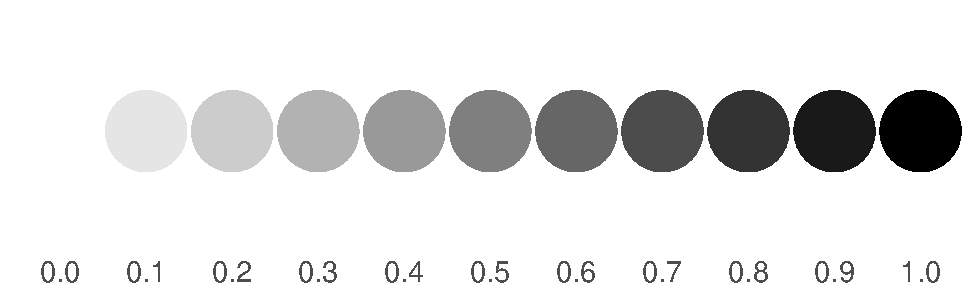
\includegraphics[width=0.5\linewidth]{contrast_and_scatterplots_files/figure-latex/formal-contrast-1} \hfill{}

\caption{\label{formal-contrast}Higher alpha values result in greater contrast between the foreground (scatterplot point) and background. When alpha = 0, the foreground is ignored and the background is rendered.}\label{fig:formal-contrast}
\end{figure}

\hypertarget{overview-of-experiments}{%
\subsection{Overview of Experiments}\label{overview-of-experiments}}

Experiments 1 and 2 share multiple aspects of their procedures. Both
experiments were built using PsychoPy \citep{pierce_psychopy_2019}, and
hosted on pavlovia.org. Both use 1-factor, 4-level designs. Participants
were only permitted to complete the experiments on a desktop computer or
laptop. As with the luminances of scatterplots and their points, our
crowd-sourced approach renders the measurement of participant-to-monitor
distance and the recording of exact apparatus impossible. We do not
consider this a shortcoming however, as it allows for findings that are
robust to various displays and viewing contexts and allows us to make
conclusions that are of particular relevance to the HCI audience.

Ethical approval for both experiments was granted by the University of
Manchester's Computer Science Department Panel (Ref: 2022-14660-24397).
Each participant was shown the participant information sheet (PIS) and
provided consent through key presses in response to consent statements.
They were then asked to provide their age in a free text box, and their
gender identity. Following this they were asked to complete the 5-item
Subjective Graph Literacy (SGL) test \citep{garcia_2016}. Participants
were then shown 7 instructional slides that can be seen in the
experimental repository
(https://gitlab.pavlovia.org/Strain/exp\_uniform\_adjustments/blob/master/instructions.csv).
Ad-hoc piloting with a graduate student in humanities suggested people
might be unfamiliar with what different correlations looked like in
scatterplots. They were therefore shown examples of \emph{r} = 0.2, 0.5,
0.8, and 0.95, which can be see in Figure \ref{example-plots}.
Participants were then given two practice trials before the experiment
began.

\begin{figure}

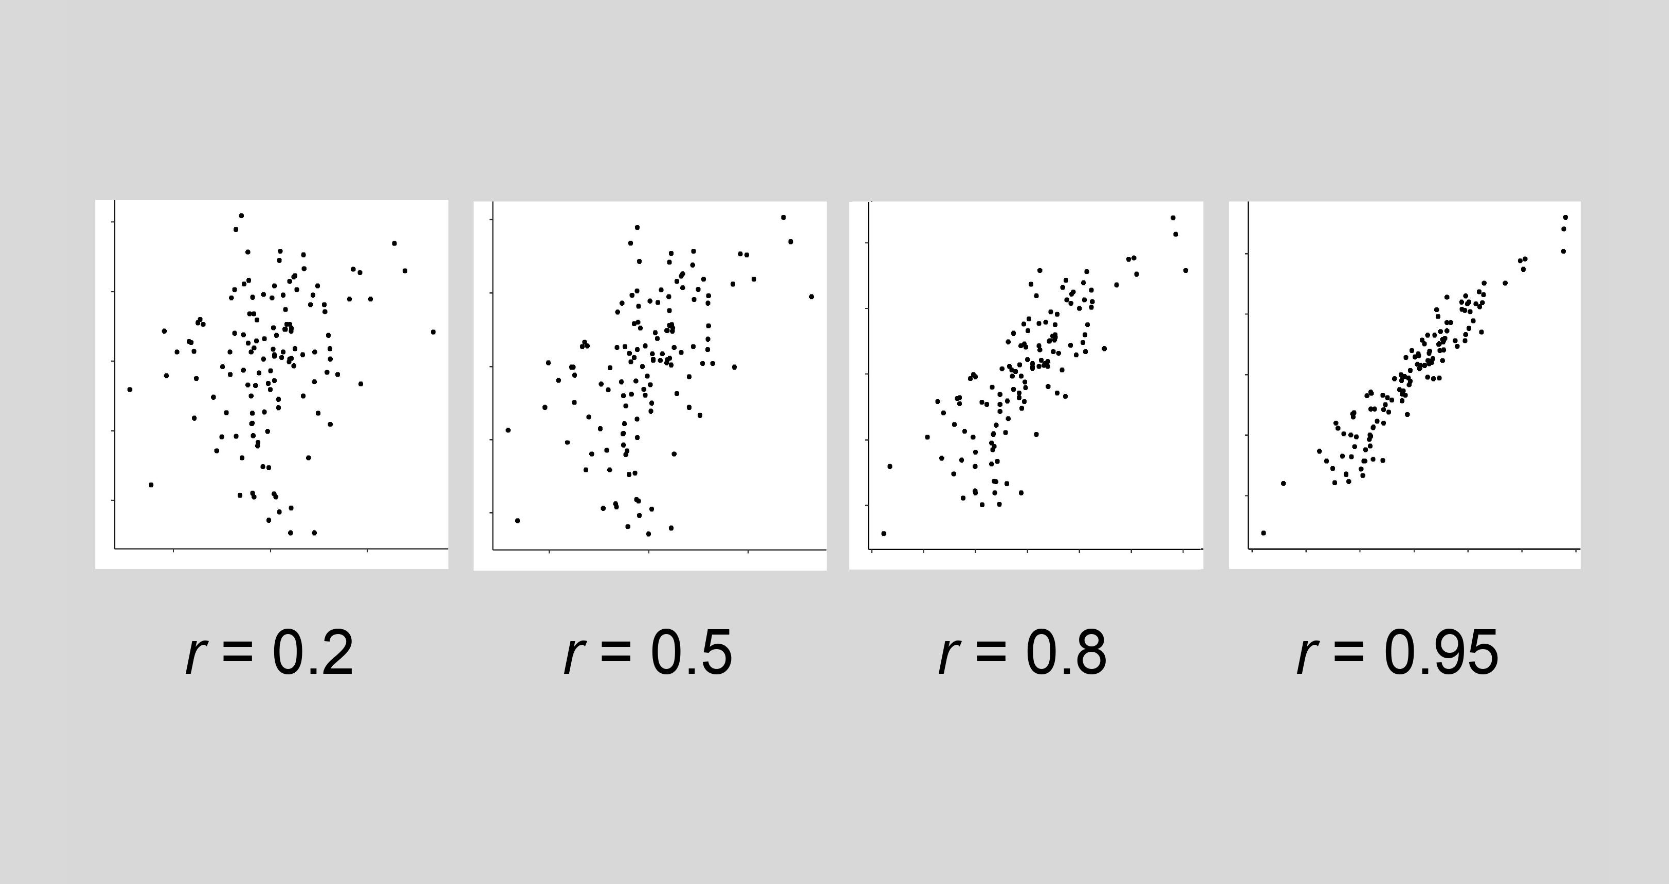
\includegraphics[width=0.5\linewidth]{images/example-plots} \hfill{}

\caption{\label{example-plots}Participants viewed this for at least 8 seconds before being allowed to continue onto the practice trials.}\label{fig:example-plots}
\end{figure}

Each trial was preceded by text that either told the participant
``Please look at the following plot and use the slider to estimate the
correlation'' (in black, experimental trial), or ``Please IGNORE the
correlation displayed and set the slider to 1''\footnote{The word
  ``ignore'' was in lowercase in the first experiment, but was changed
  to uppercase in the second to increase the salience of attention check
  items.} (n = 3) or ``Please IGNORE the correlation displayed and set
the slider to 0''\footnote{The word ``ignore'' was in lowercase in the
  first experiment, but was changed to uppercase in the second to
  increase the salience of attention check items.} (n = 3) (in red,
attention check trial). Each plot was preceded by a visual mask
displayed for 2.5 seconds. Figure \ref{example-trial} shows an example
of an experimental trial. There was no time limit per trial, but
participants were instructed to make their judgements as accurately and
quickly as possible.

Both experiments described here use a fully repeated measures,
within-participants design. Participants saw all 180 plots,
corresponding to \textasciitilde{} 27,000 individual judgements per
experiment. Presentation order was randomised.

\begin{figure}

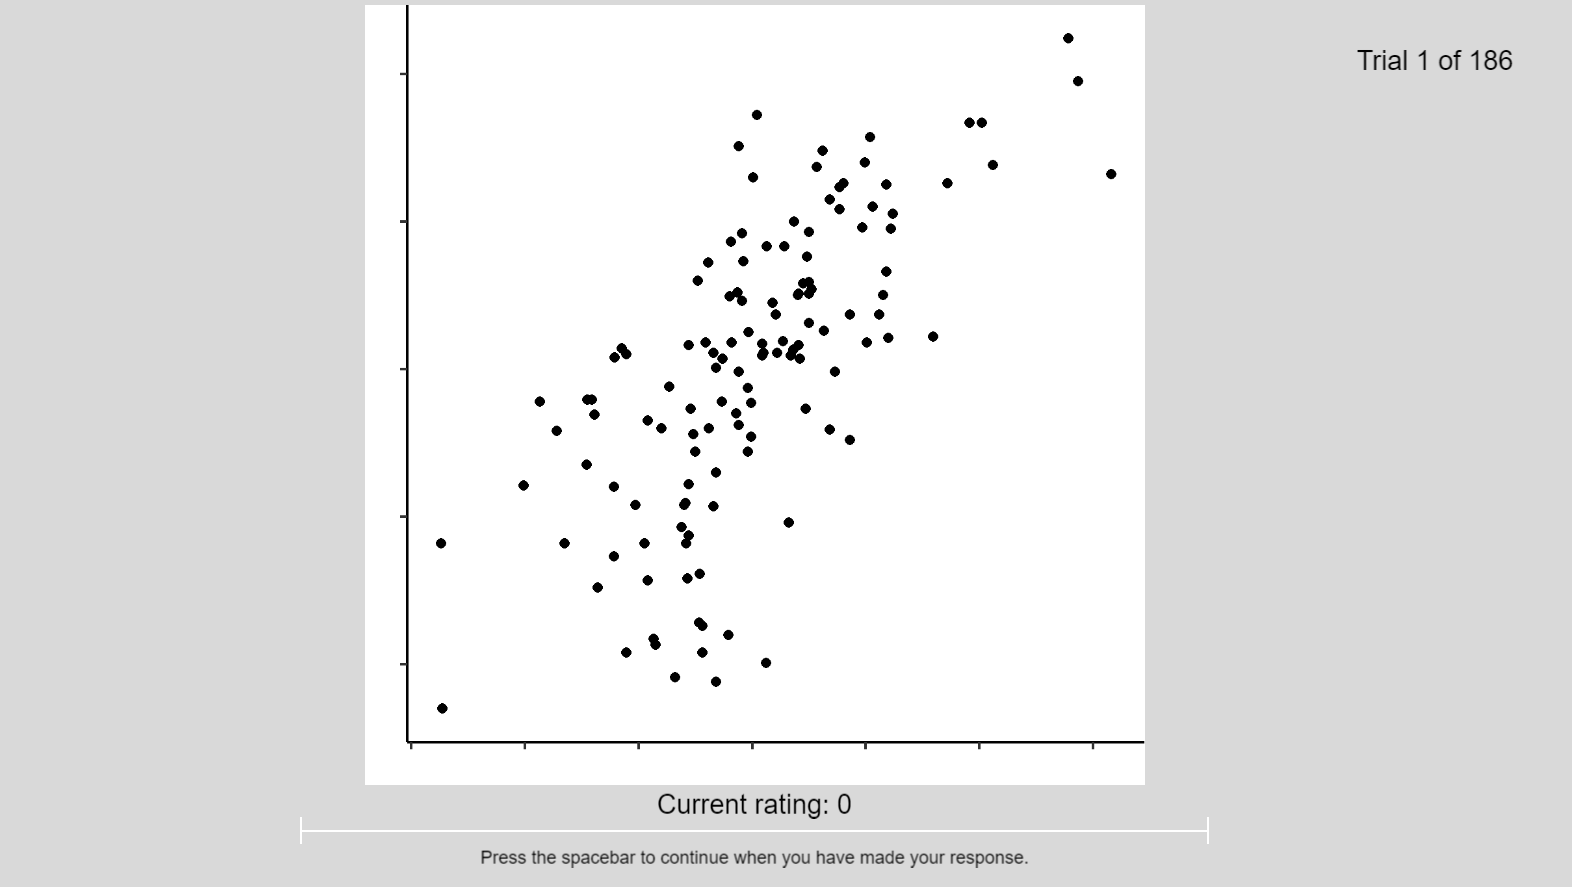
\includegraphics[width=0.5\linewidth]{images/example-trial} \hfill{}

\caption{\label{example-trial}An example of an experimental trial.}\label{fig:example-trial}
\end{figure}

\hypertarget{plot-generation}{%
\subsection{Plot Generation}\label{plot-generation}}

Scatterplots were randomly generated from bivariate normal
distributions. All plots presented were 1200 * 1200 pixels in size, and
included no titles, tick labels, or axis labels. Points were 10 pixels
in diameter on a 1280x720 resolution monitor, and 13 pixels in diameter
on a 1920x1080 resolution monitor. Due to our crowdsourced approach we
were unable to obtain precise monitor resolution or physical screen size
measurements for participants, meaning we are unable to provide
by-participant dot pitch information. We are however working on a method
to accomplish this in future work. Each plot contained 128 data points.
45 \emph{r} values were generated on a uniform distribution between 0.2
and 0.95. We chose these boundaries due to evidence that very little
correlation is perceived below 0.2
\citep{bobko_1979, cleveland_1982, strahan_1978}. Scatterplots were
generated according to the standard normal distribution, having a
standard deviation of 1 in each direction. Scripts detailing item and
mask creation for each experiment can be found in the item\_preparation
folder.

\hypertarget{open-research-statement}{%
\section{Open Research Statement}\label{open-research-statement}}

Both experiments were conducted according to the principles of open and
reproducible research. All data and analysis code are available at
https://github.com/gjpstrain/contrast\_and\_scatterplots. This
repository contains instructions for building a Docker container that
fully reproduces the computational environment this paper was written
in, allowing for a full recreation of both stimulus generation and the
paper itself. Both experiments and their related hypotheses and analysis
plans were pre-registered with the OSF (https://osf.io/v23e9/), and
there were no deviations from them. We used linear mixed-effects models
to model the relationships between our independent variables (point
contrast in experiment 1 and the type of contrast decay function in
experiment 2) and our dependent variable (participants' estimates of
correlation). Linear mixed-effects models allow us to compare difference
between levels of our independent variable across the full range of
participant responses on the dependent variable, as opposed to simply
analysing the differences between means that would be afforded to us
with ANOVA. Linear mixed-effects models also allow us to include random
effects for both participants and experimental items in our modelling.
Consistent with our pre-registrations, we aimed for the most complex
random effects structures when producing models. The structure of these
models was identified using the \textbf{buildmer} package in R
\citep{voeten_buildmer_2022}. This package takes the most complex random
effects model, in terms of intercepts for participants and items and
corresponding slopes for fixed effects terms as an input. It then
identifies the most complex model that successfully converges, dropping
terms that fail to explain a significant amount of variance, as assessed
with likelihood ratio tests. This provides a simple and reproducible
methodology for the construction of linear mixed-effects models. This
approach does mean that the final model used is not always the most
complex one possible, but rather is the most complex that substantially
explains variance and converges.

\hypertarget{experiment-1-changing-the-contrast-of-all-points}{%
\section{Experiment 1: Changing the Contrast of All
Points}\label{experiment-1-changing-the-contrast-of-all-points}}

\hypertarget{introduction-1}{%
\subsection{Introduction}\label{introduction-1}}

Our first experiment varied the contrast of every point on a scatterplot
in a uniform manner. Given the effects of contrast on perception
described above \citep{champion_2017, wehrhahn_1990}, we hypothesized
that there would be a more variable spread of correlation estimates for
plots with lower contrast compared to plots with higher contrast,
potentially due to the greater spatial uncertainty induced by lower
contrast.

\hypertarget{method}{%
\subsection{Method}\label{method}}

\hypertarget{participants}{%
\subsubsection{Participants}\label{participants}}

150 participants were recruited using the Prolific.co platform. Normal
to corrected-to-normal vision and English fluency were required for
participation. In accordance with guidelines published in
\citet{peer_2021}, participants were required to have previously
completed at least 100 studies on Prolific, and were required to have a
Prolific score of at least 100, indicating acceptance on at least
100/101 studies previously completed. In addition, participants who had
completed an earlier, similar study that was run by the authors of the
current paper, were prevented from participating.

Data were collected from 158 participants. 8 failed more than 2 out of 6
attention check questions, and, as per pre-registration stipulations,
were rejected from the study. The remaining 150 participants' data were
included in the full analysis (51.01\% male, 47.65\% female, and 1.34\%
non-binary). Mean age of participants was 28.29 (\emph{SD} = 8.59). Mean
graph literacy score was 21.76 (\emph{SD} = 4.47) out of 30. The average
time taken to complete the experiment was 33 minutes (SD = 10 minutes).

\hypertarget{design}{%
\subsubsection{Design}\label{design}}

For each of the 45 \emph{r} values there were 4 versions of each plot
corresponding to the 4 levels of point contrast, examples of which can
be seen in Figure \ref{e1-example-plots}.

The experiment is hosted at
https://gitlab.pavlovia.org/Strain/exp\_uniform\_adjustments. This
repository contains all the experimental code, materials, and
instructions needed to run the experiment in full.

\begin{figure}

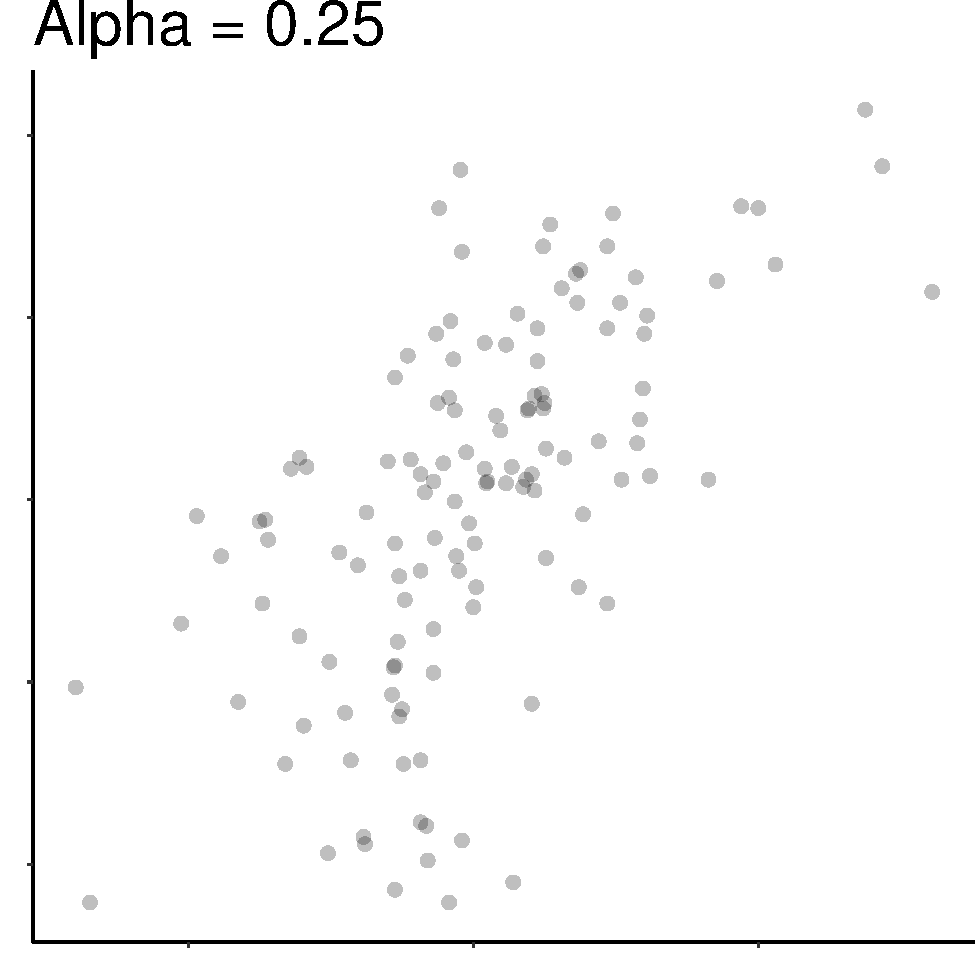
\includegraphics[width=0.5\linewidth]{contrast_and_scatterplots_files/figure-latex/e1-example-plots-1} 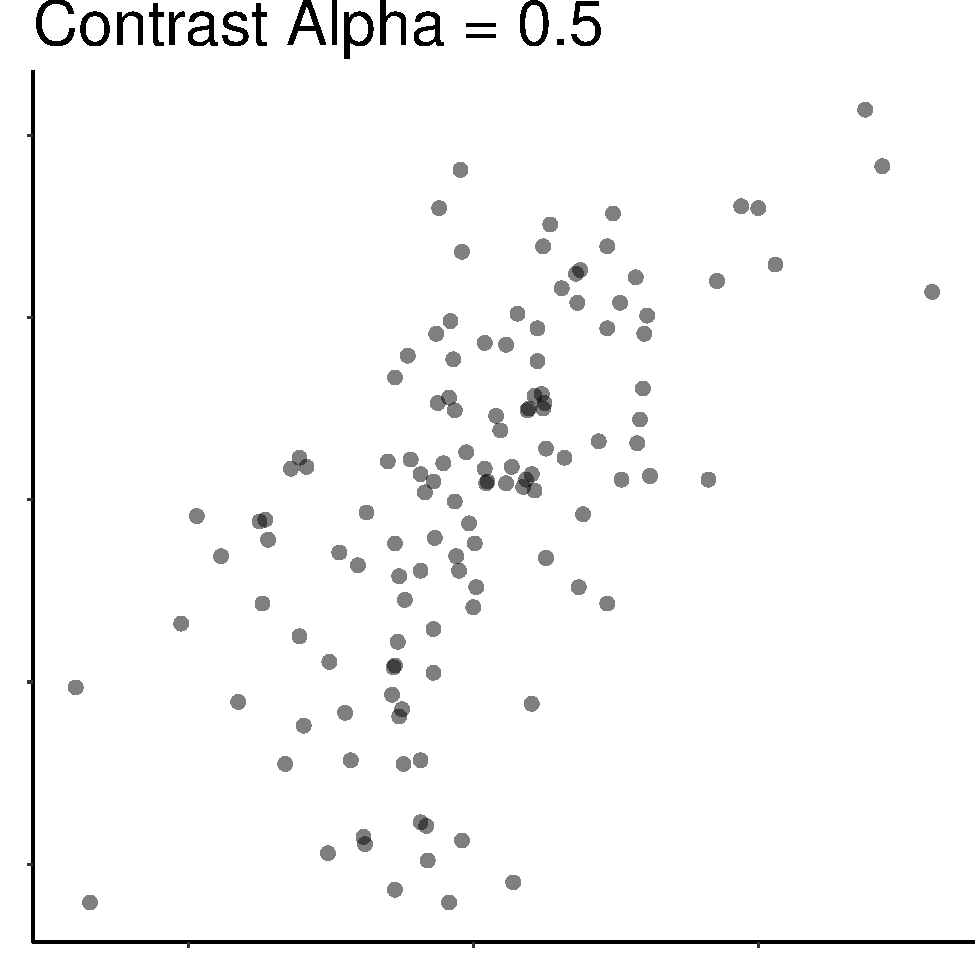
\includegraphics[width=0.5\linewidth]{contrast_and_scatterplots_files/figure-latex/e1-example-plots-2} 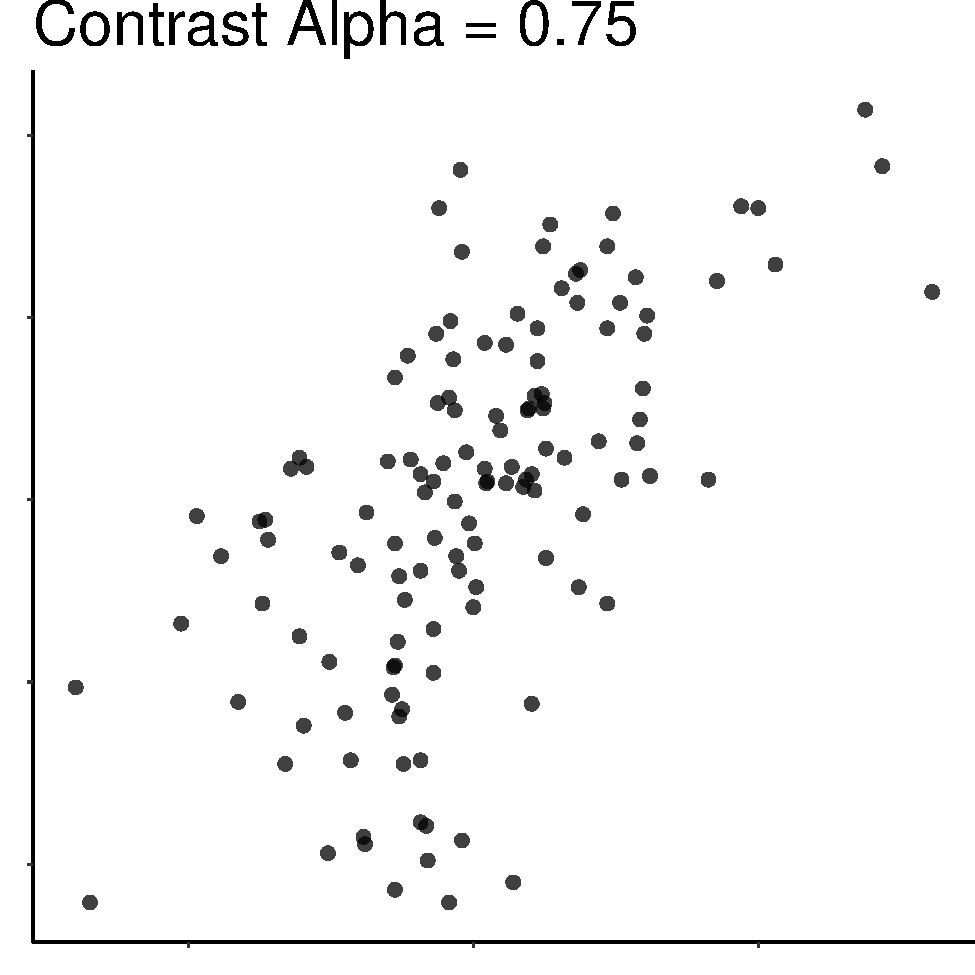
\includegraphics[width=0.5\linewidth]{contrast_and_scatterplots_files/figure-latex/e1-example-plots-3} 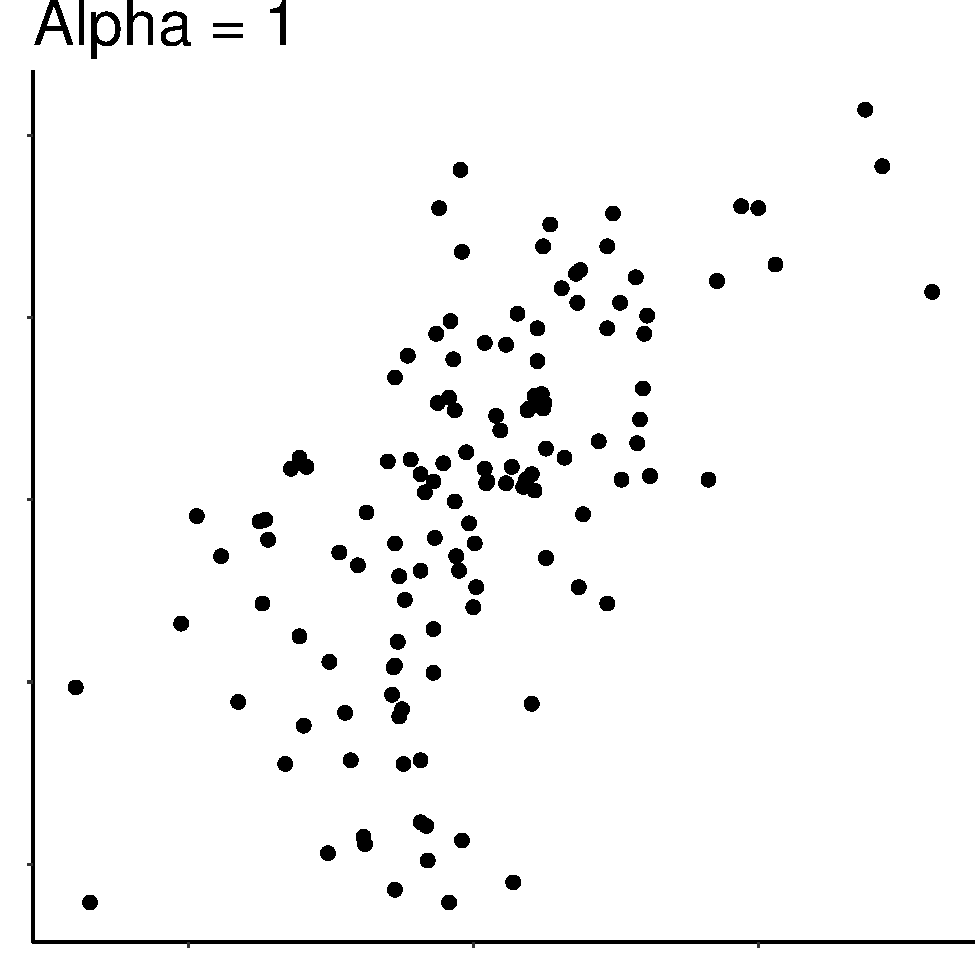
\includegraphics[width=0.5\linewidth]{contrast_and_scatterplots_files/figure-latex/e1-example-plots-4} \hfill{}

\caption{\label{e1-example-plots}The four levels of the contrast condition in experiment 1, demonstrated with an \textit{r} value of 0.6.}\label{fig:e1-example-plots}
\end{figure}

\hypertarget{results}{%
\subsection{Results}\label{results}}

All analyses were conducted using R (version 4.2.1, \citep{r_core}).
Models were built using the \textbf{buildmer} (version 2.7
\citep{voeten_buildmer_2022}) and \textbf{lme4} (version 1.1-30
\citep{bates_lme4_2015}) packages.

\begin{figure}

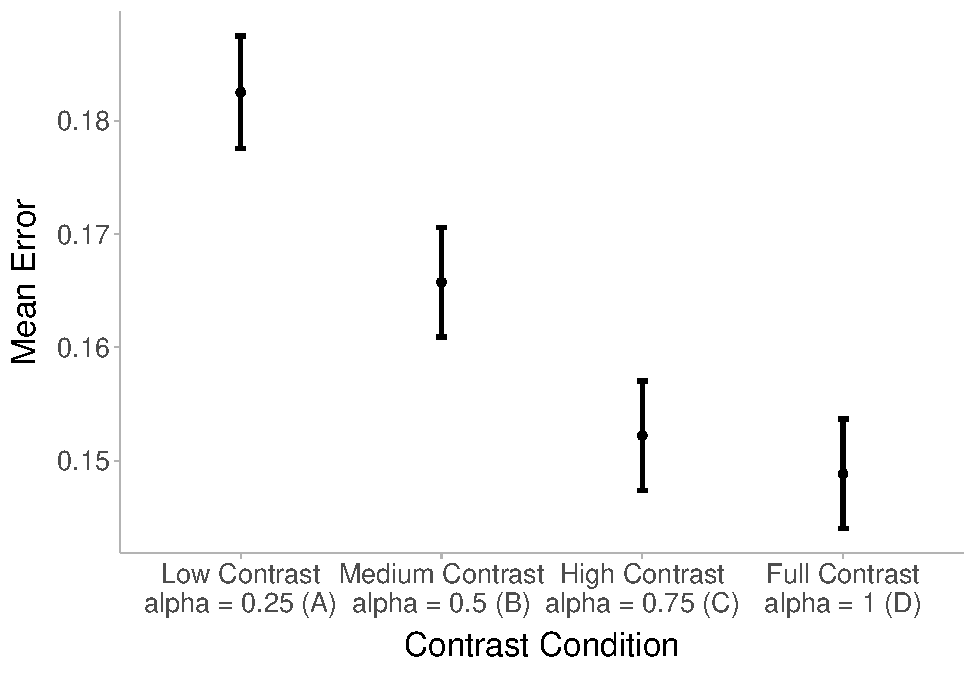
\includegraphics[width=0.5\linewidth]{contrast_and_scatterplots_files/figure-latex/e1-dot-plot-1} \hfill{}

\caption{\label{e1-dot-plot}Mean error in correlation estimation across the four contrast conditions in E1, with 95\% confidence intervals shown.}\label{fig:e1-dot-plot}
\end{figure}

Figure \ref{e1-dot-plot} shows the mean error in correlation estimation
for the 4 contrast conditions. A likelihood ratio test reveals that the
model including contrast as a fixed effect explained significantly more
variance than a model not including contrast as a fixed effect
(\(\chi^2\)(3) = 224.25, \emph{p} \textless{} .001). This model has
random intercepts for items and participants. This effect was driven by:
low contrast scatterplots (contrast alpha = 0.25) being rated on average
as having lower correlation than medium contrast (contrast alpha = 0.5),
high contrast (contrast alpha = 0.75), and full contrast (contrast alpha
= 1) plots; and medium contrast plots being rated on average as having
lower correlation than high and full contrast plots. There was no
significant difference in correlation estimates between high and full
contrast plots.

Statistical testing for contrasts between the 4 levels of the contrast
condition was performed with the \textbf{emmeans} package (version
1.8.1-1, \citep{emmeans}) and are shown in table
\ref{contrasts-table-e1}. Means and 95\% confidence intervals of
correlation judgements are shown in figure \ref{e1-dot-plot}. The
\textbf{EMAtools} package (version 0.1.4 \citep{ematools}) was used to
calculate effect sizes in Cohen's d.~For the difference in correlation
ratings between the lowest contrast (alpha = 0.25) and highest contrast
plots (alpha = 1), an effect size of d = -0.08 was obtained. While this
effect is small, it is not insignificant, and given the lack of reported
effect on correlation perception of global point contrast adjustments
\citep{rensink_2012} is an unsurprising result.

\begin{table}

\caption{\label{tab:contrasts-table-e1}\label{contrasts-table-e1}This table shows the contrasts between different levels of the contrast factor in E1.}
\centering
\begin{tabular}[t]{lrl}
\toprule
Contrast & Z.ratio & p.value\\
\midrule
Low contrast (A) : Full contrast (D) & 13.48 & <0.001\\
Low contrast (A) : High contrast (C) & 12.12 & <0.001\\
Low contrast (A) : Medium contrast (B) & 6.72 & <0.001\\
Full contrast (D) : High contrast (C) & -1.35 & 0.528\\
Full contrast (D) : Medium contrast (B) & -6.76 & <0.001\\
\addlinespace
High contrast (C) : Medium contrast (B) & -5.40 & <0.001\\
\bottomrule
\end{tabular}
\end{table}

We also generate an additional model to test whether the results we
found could be explained by differences in graph literacy. This model is
identical to the experimental one, but includes graph literacy as a
fixed effect. We found no significant differences between the original
model and the one including graph literacy as a fixed effect
(\(\chi^2\)(1) \textless{} .001, \emph{p} = .995). These results suggest
that the effect we found was not driven by differences in graph literacy
between participants.

\begin{figure}

{\centering 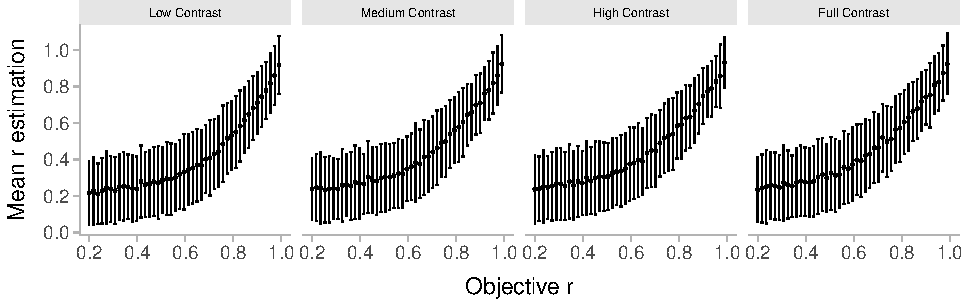
\includegraphics{contrast_and_scatterplots_files/figure-latex/e1-error-plot-1} 

}

\caption{\label{e1-error-plot}The mean of participants' estimations of \textit{r} compared with objective Pearson's \textit{r}, plotted by contrast condition. Error bars show standard deviations of mean estimates.}\label{fig:e1-error-plot}
\end{figure}

Figure \ref{e1-error-plot} shows how participants' mean estimates of
correlation change with the objective Pearson's \emph{r} value, plotted
separately for each contrast condition. We observe underestimation
curves similar to those reported in previous literature (see section
\ref{testing}).

\hypertarget{discussion}{%
\subsection{Discussion}\label{discussion}}

\begin{figure}

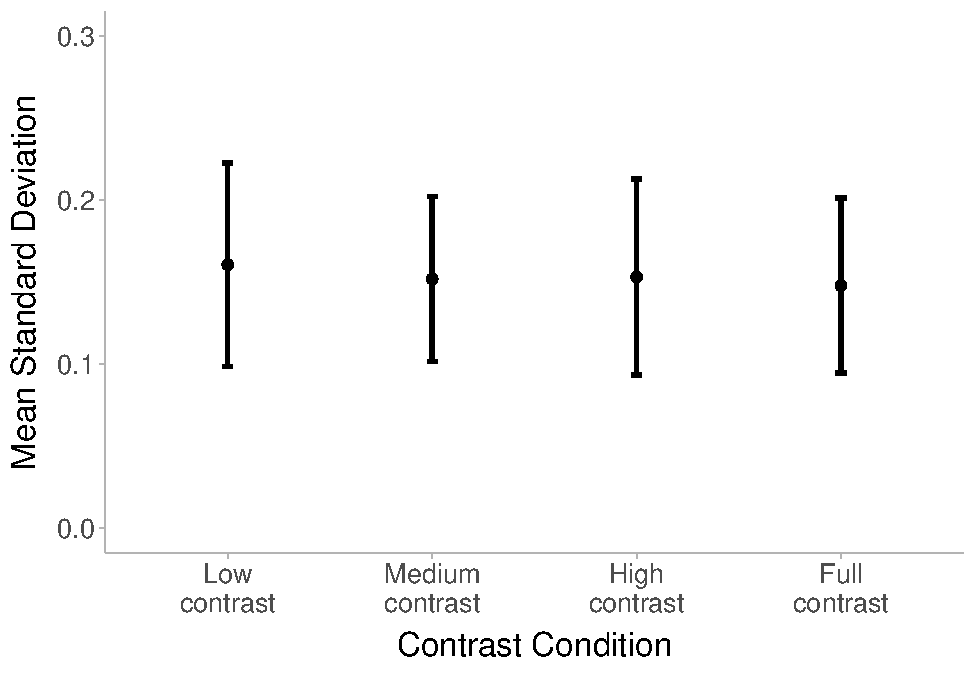
\includegraphics[width=0.5\linewidth]{contrast_and_scatterplots_files/figure-latex/e1-sd-sd-plot-1} \hfill{}

\caption{\label{e1-sd-sd-plot}The mean of standard deviations of participants in experiment 1, grouped by contrast condition.}\label{fig:e1-sd-sd-plot}
\end{figure}

Our hypothesis was not supported in this experiment. We hypothesized
that plots with lower contrast would have a more variable spread of
correlation estimates than plots with higher contrast. As shown in
figure \ref{e1-sd-sd-plot}, there was little difference in mean standard
deviations between the 4 contrast conditions. Participants' errors in
correlation estimation were significantly higher when the contrast of
all points was lower compared to when it was higher. This was true up
until contrast alpha was set to 0.75, implying a threshold around alpha
= 0.75 past which there is little variation in the perception of
contrast, at least as far as it is associated with correlation
estimation. This lack of significant difference in correlation
estimation between our two highest contrast values fits with the
logarithmic nature of contrast/brightness perception
\citep{varshney_2013, fechner_1948}; despite there being equal linear
distance between the contrast values we used, the perceptual distance
between them was clearly non-linear.

As mentioned previously, \citet{rensink_2012} and \citet{rensink_2014}
describe what is, to our knowledge, the only other direct testing of
correlation perception and point contrast, and reports invariance in
accuracy and precision with regards to contrast. Our results contradict
these previously reported findings, which we argue is due to crucial
differences in methodology and experimental power. Rensink used
bisection and JND tasks to fit equations for accuracy and precision. Our
methodology simply asked participants to estimate correlation, producing
comparative judgements more suited to informing scatterplot design than
the absolute relationship between correlation and perceived correlation
illuminated upon by other methodologies. The major strength of this
study is the large sample size (n = 150). Compared with the relatively
small sample size in \citet{rensink_2014} (n = 12), our study's
heightened experimental power represents strong evidence that total
contrast in a scatterplot can affect people's perceptions of
correlation. Our effect size for the uniform contrast manipulation was
small (d = -0.08), and while such a small difference may be of little
practical relevance , it demonstrates that differences in the contrast
of points can effect correlation estimates in scatterplots. The fact
that this difference is present suggests that it can be used to optimise
perception, which we start attempting to do in experiment two. We
suggest that correlation perception functions similarly to speed
perception \citep{champion_2017} with regards to changes in contrast;
the greater spatial uncertainty brought on by reduced contrast, while
not eliciting the greater spread in correlation estimates that we
hypothesized, might be responsible for the results observed via an
increase in the perceived width of the probability distribution in the
plot.

From our results it is clear that a scatterplot optimized for
correlation perception should have maximum contrast between the
foreground (points) and background. That we found significant
differences in correlation estimation between data-identical
scatterplots with different point contrasts however, suggests that we
might be able to leverage this effect to further improve participants'
estimates of correlation.

\hypertarget{experiment-2-spatially-dependent-contrast-adjustments}{%
\section{Experiment 2: Spatially-Dependent Contrast
Adjustments}\label{experiment-2-spatially-dependent-contrast-adjustments}}

\hypertarget{introduction-2}{%
\subsection{Introduction}\label{introduction-2}}

In experiment 1 we found that contrast has a clear effect on the
perception of correlation such that scatterplots with higher levels of
point contrast are rated as being more correlated. Given this result,
the important question arises of whether we might see additional changes
in correlation perception as a function of the spatial arrangement of
point contrast in scatterplots. With this question in mind, we
hypothesized that participants' estimates of correlation would exhibit
lower mean error with the decay parameter in which contrast falls with
residual distance in a non-linear fashion (the non-linear decay
parameter), and that the use of a non-linear inverted decay parameter,
in which contrast increased with residual distance, would result in
higher mean errors than all other conditions.

\hypertarget{methods}{%
\subsection{Methods}\label{methods}}

\hypertarget{participants-1}{%
\subsubsection{Participants}\label{participants-1}}

150 participants were recruited using the Prolific.co platform. Normal
to corrected-to-normal vision and English fluency were required for
participation. In accordance with guidelines published in
\citep{peer_2021}, participants were required to have previously
completed at least 100 studies on Prolific, and were required to have a
Prolific score of at least 100, indicating acceptance on at least
100/101 previously completed studies. In addition, participants who had
completed an earlier, similar study that was run by the authors of the
current paper, or the first experiment described above were prevented
from participating.

Data were collected from 157 participants. 7 failed more than 2 out of 6
attention check questions, and, as per pre-registration stipulations,
were rejected from the study. The remaining 150 participants data were
included in the full analysis (51.33\% male, 46.00\% female, and 2.67\%
non-binary). Mean age of participants was 27.05 (\emph{SD} = 7.37). Mean
graph literacy score was 21.71 (\emph{SD} = 4.06) out of 30. The average
time taken to complete the experiment was 33 minutes (SD = 13 minutes).

\hypertarget{design-1}{%
\subsubsection{Design}\label{design-1}}

For each of the 45 \emph{r} values there were four versions of each
plot, which can be seen in Figure \ref{e2-example-plots}. Three used
functions relating point residuals to point contrast, which we refer to
as decay parameters, with the remaining condition being the contrast
alpha = 1 uniform contrast condition from the first experiment. We used
the following equation to non-linearly map residuals to alpha values,
where R is the residual of the point in question. 0.25 was chosen as the
value of \(b\). Given the shape of the underestimation curve reported in
previous literature (see figure \ref{underestimation-curve}), intuition
suggested that we use a symmetrically opposing curve (see figure
\ref{decay-parameters}) to relate point contrast with residuals. We
tested a number of values of \(b\), and felt that 0.25 rendered plots
that maintained point legibility while also allowing a large enough
range in contrast that, if an effect was present, one would be found.

\begin{align}
  alpha = 1 - b^R
\end{align}

\begin{figure}

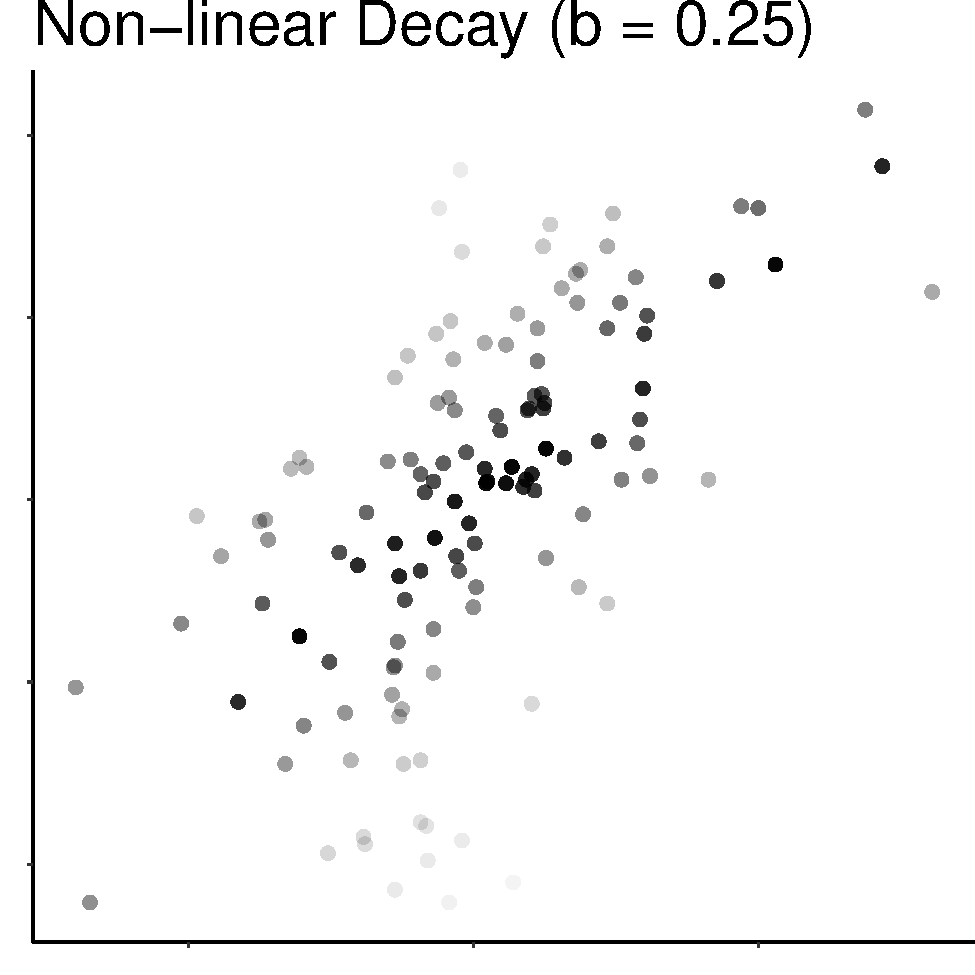
\includegraphics[width=0.5\linewidth]{contrast_and_scatterplots_files/figure-latex/e2-example-plots-1} 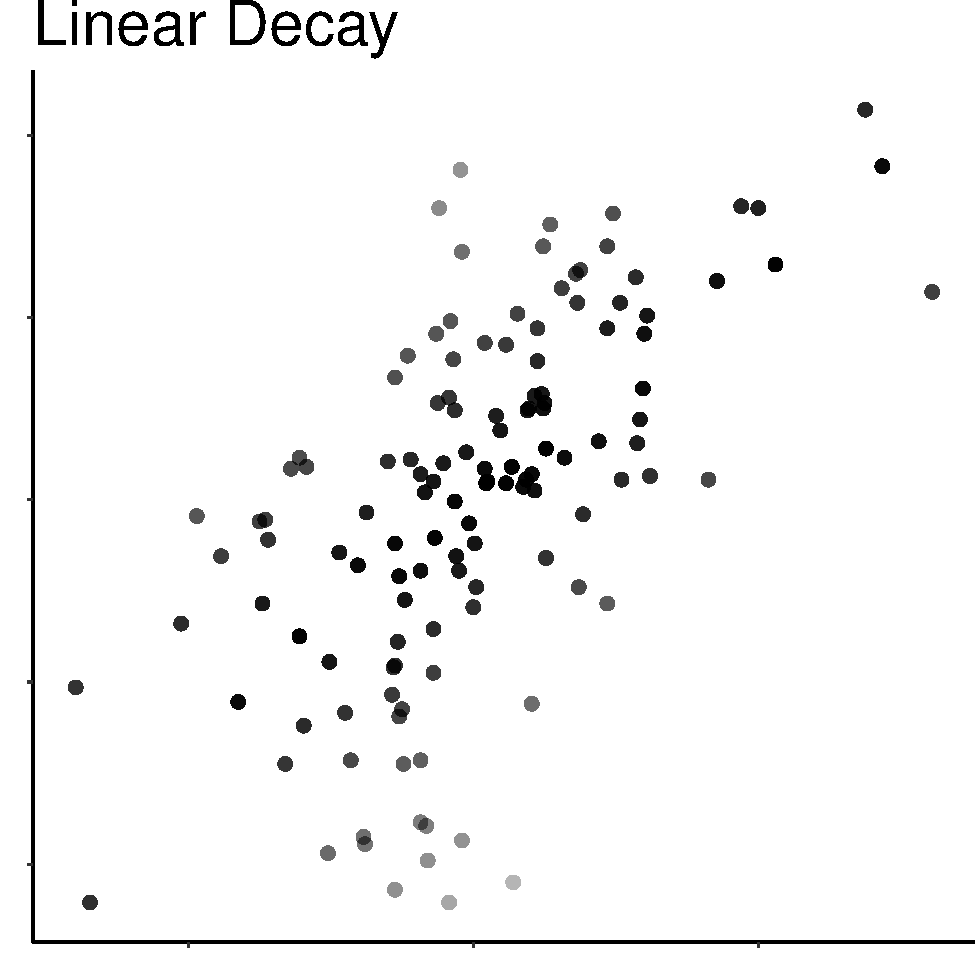
\includegraphics[width=0.5\linewidth]{contrast_and_scatterplots_files/figure-latex/e2-example-plots-2} 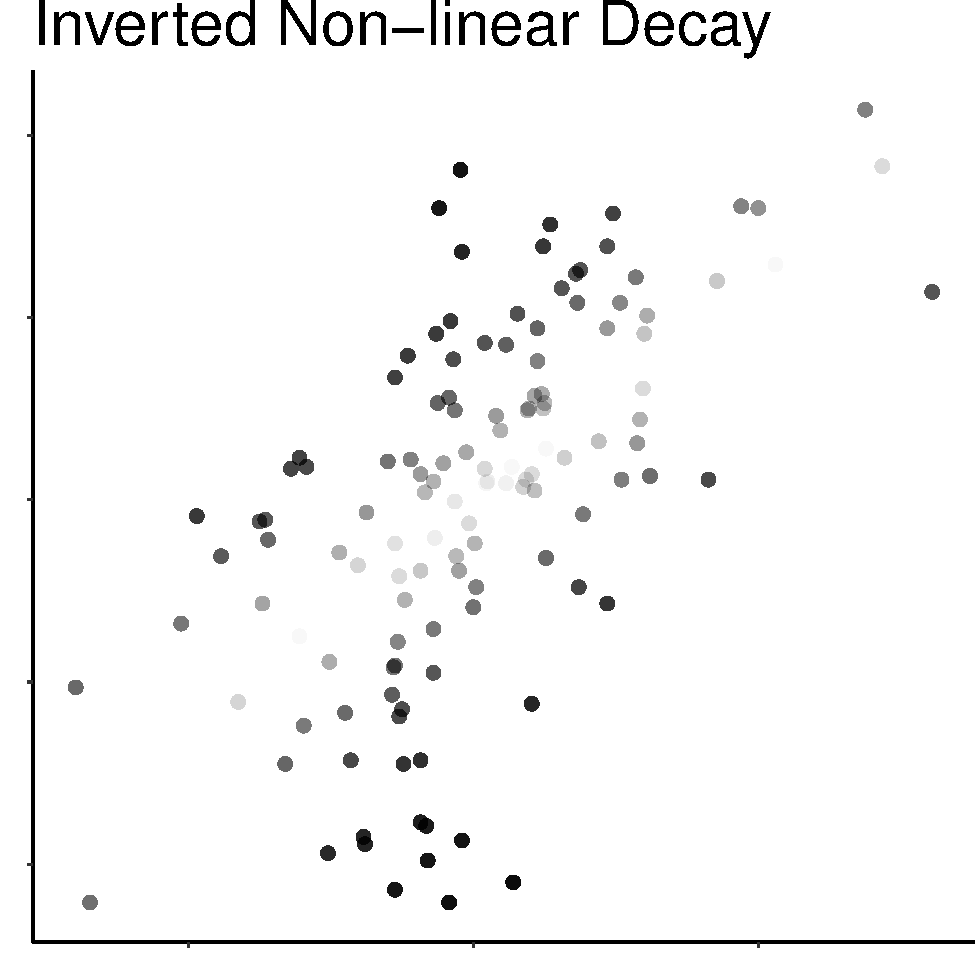
\includegraphics[width=0.5\linewidth]{contrast_and_scatterplots_files/figure-latex/e2-example-plots-3} 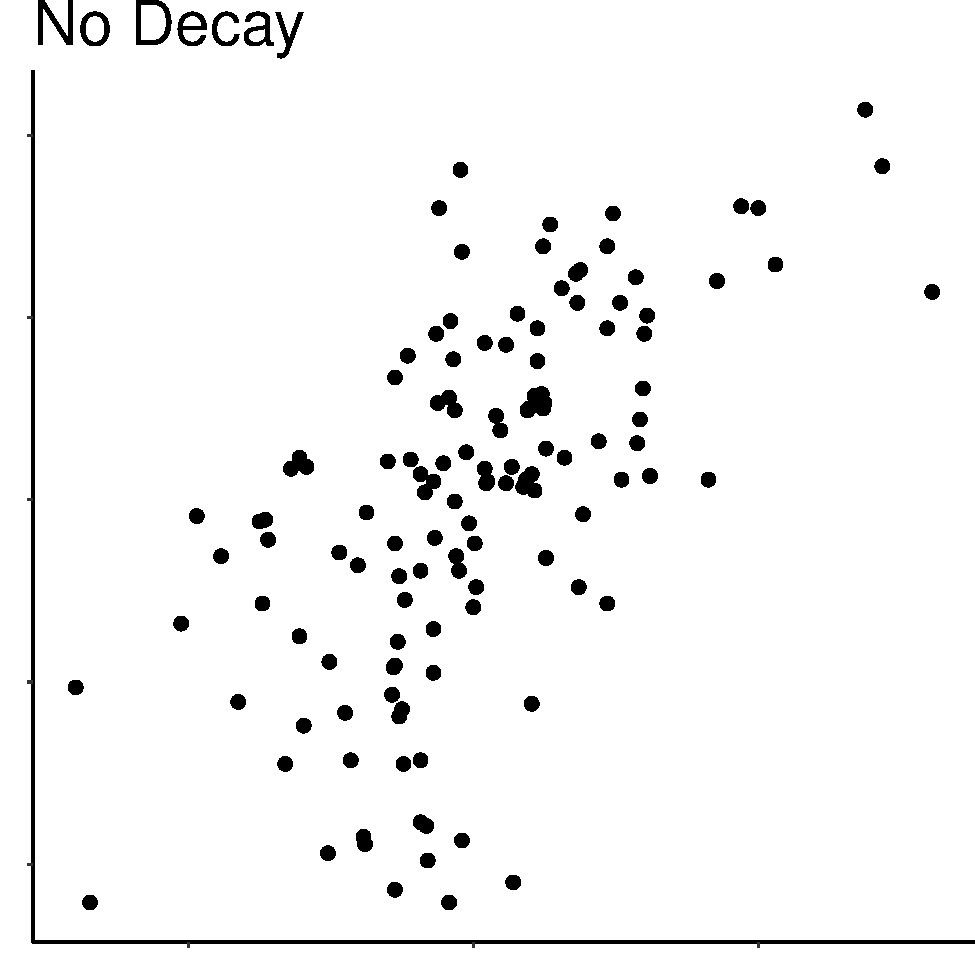
\includegraphics[width=0.5\linewidth]{contrast_and_scatterplots_files/figure-latex/e2-example-plots-4} \hfill{}

\caption{\label{e2-example-plots}The 4 levels of the contrast condition in experiment 2, demonstrated with an \textit{r} value of 0.6.}\label{fig:e2-example-plots}
\end{figure}

Figure \ref{decay-parameters} illustrates the relationship between the
size of a residual and the contrast produced.

The experiment is hosted at
https://gitlab.pavlovia.org/Strain/exp\_spatially\_dependent. This
repository contains all the experimental code, materials, and
instructions needed to run the experiment in full.

\begin{figure}
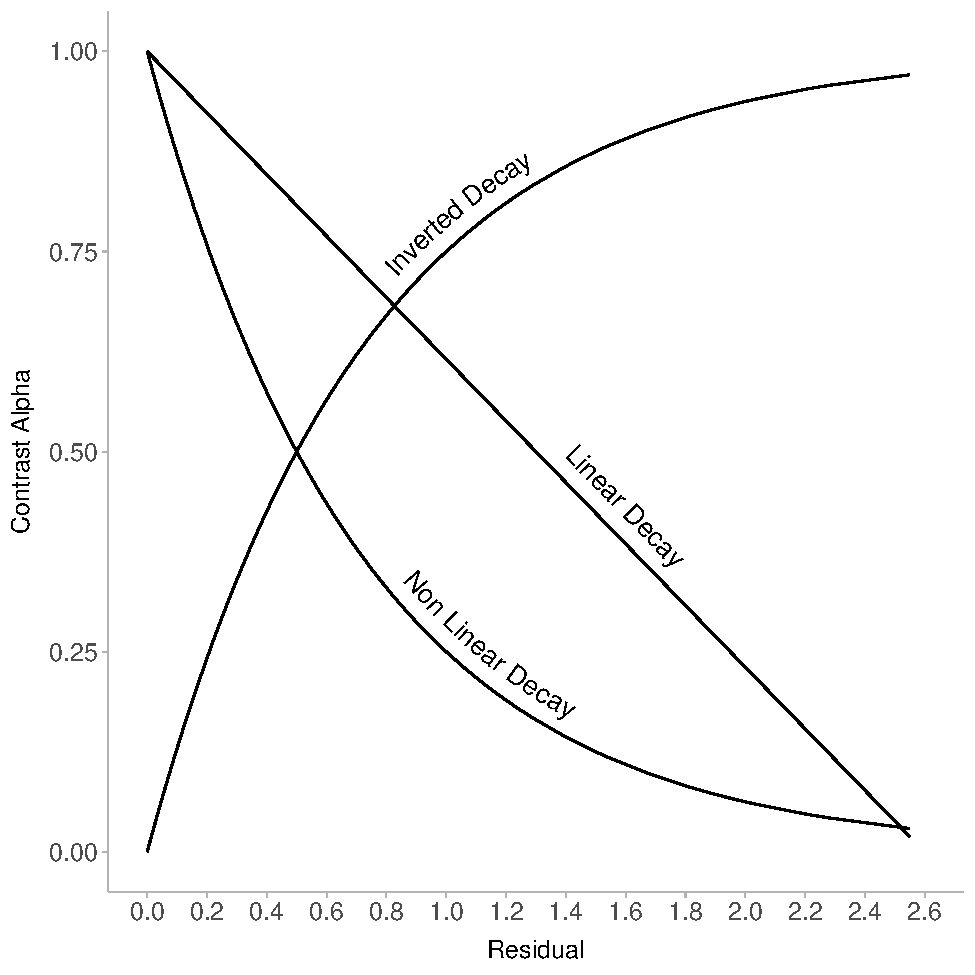
\includegraphics[width=1\linewidth]{contrast_and_scatterplots_files/figure-latex/decay-parameters-1} \caption{\label{decay-parameters}Here we use an \textit{r} value of 0.2 to demonstrate the relationship between the size of a point's residual and the contrast alpha value that translates to.}\label{fig:decay-parameters}
\end{figure}

\hypertarget{results-1}{%
\subsection{Results}\label{results-1}}

All analyses were conducted using R (version 4.2.1, \citep{r_core}) As
in E1, models were built using the \textbf{buildmer} (version 2.7,
\citep{voeten_buildmer_2022}) and \textbf{lme4} (version 1.1-30
\citep{bates_lme4_2015}) packages.

\begin{figure}

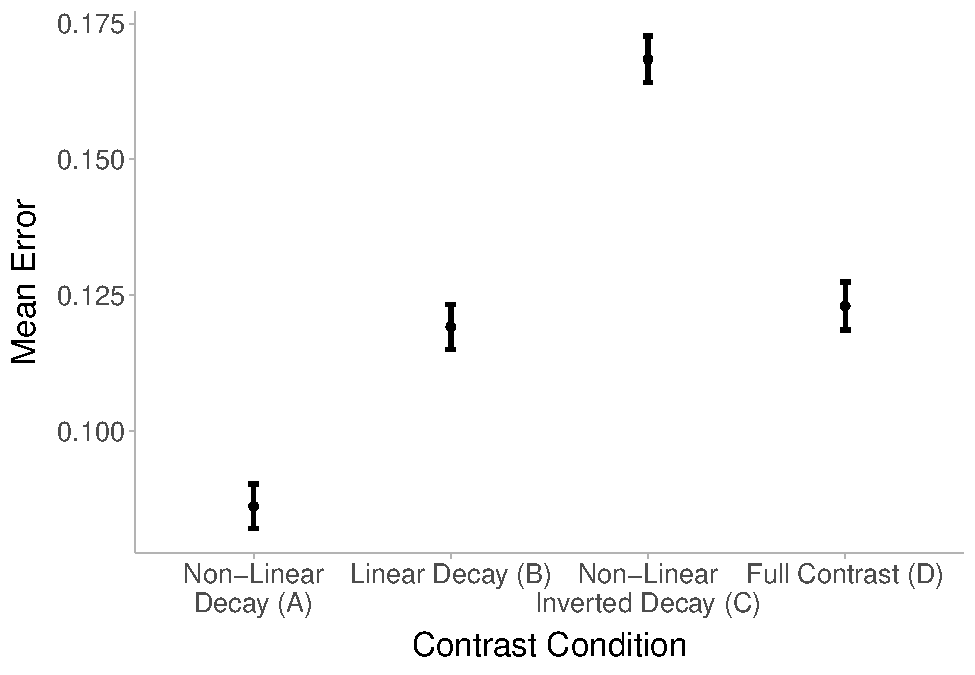
\includegraphics[width=0.5\linewidth]{contrast_and_scatterplots_files/figure-latex/e2-dot-plot-1} \hfill{}

\caption{\label{e2-dot-plot}Mean error in correlation estimation across the four contrast conditions in E2, with 95\% confidence intervals shown}\label{fig:e2-dot-plot}
\end{figure}

Figure \ref{e2-dot-plot} shows mean correlation estimation errors for
the 4 contrast conditions. A likelihood ratio test reveals that the
model including contrast condition as a fixed effect explained
significantly more variance than a model not including contrast as a
fixed effect (\(\chi^2\)(3) = 1,157.62, \emph{p} \textless{} .001). This
model has random intercepts for items and participants. This effect was
driven by participants' correlation estimates being on average more
accurate for the non-linear decay parameter than for the linear decay
parameter, non-linear inverted decay parameter, and full contrast
conditions; by estimates with linear decay being more accurate than
estimates with non-linear inverted decay; and by full contrast estimates
being more accurate than estimates with non-linear inverted decay. There
was no significant difference in correlation estimates between linear
decay and full contrast conditions. Similar to the lack of significant
difference between high and full contrast conditions in experiment 1, we
hypothesise that this is due to the difference between these two
conditions becoming smaller as objective correlation approaches 1; it
may be that the difference is not on the whole great enough to produce a
significant effect.

Statistical testing for significant contrasts between the 4 levels of
the contrast conditions was performed with the \textbf{emmeans} package
(version 1.8.1-1, \citep{emmeans}) and are shown in table
\ref{contrasts-table-e2}. Means and 95\% confidence intervals of
correlation estimates are shown in figure \ref{e2-dot-plot}.The
\textbf{EMAtools} package (version 0.1.4 \citep{ematools}) was used to
calculate effect sizes in Cohen's d.~For the difference in correlation
ratings between full contrast and non-linear decay function plots, an
effect size of d = 0.19 was obtained. Between full contrast and
non-linear inverted decay conditions, an effect size of d = 0.17 was
obtained. These effects sizes are small and medium, but again, not
insignificant.

\begin{table}

\caption{\label{tab:contrasts-table-e2}\label{contrasts-table-e2}This table shows the contrasts between different levels of the contrast factor. A = Non-linear contrast decay (a = 0.25). B = Linear decay, C = Non-linear inverted decay, D = Full contrast.}
\centering
\begin{tabular}[t]{lrl}
\toprule
Contrast & Z.ratio & p.value\\
\midrule
Full contrast (D) : Non-linear inverted decay (C) & -18.88 & <0.001\\
Full contrast (D) : Linear decay (B) & 1.55 & 0.405\\
Full contrast (D) : Non-linear contrast decay (A) & 15.30 & <0.001\\
Non-linear inverted decay (C) : Linear decay (B) & 20.43 & <0.001\\
Non-linear inverted decay (C) : Non-linear contrast decay (A) & 34.17 & <0.001\\
\addlinespace
Linear decay (B) : Non-linear contrast decay (A) & 13.74 & <0.001\\
\bottomrule
\end{tabular}
\end{table}

Again, we also generated an additional model to test whether the results
we found could be explained by differences in graph literacy. This model
is identical to the experimental one, but includes graph literacy as a
fixed effect. We found no significant differences between the original
model and the one including graph literacy as a fixed effect
(\(\chi^2\)(1) = 0.24, \emph{p} = .623). These results suggest that the
effect we found was not driven by differences in graph literacy between
participants.

\begin{figure}

{\centering 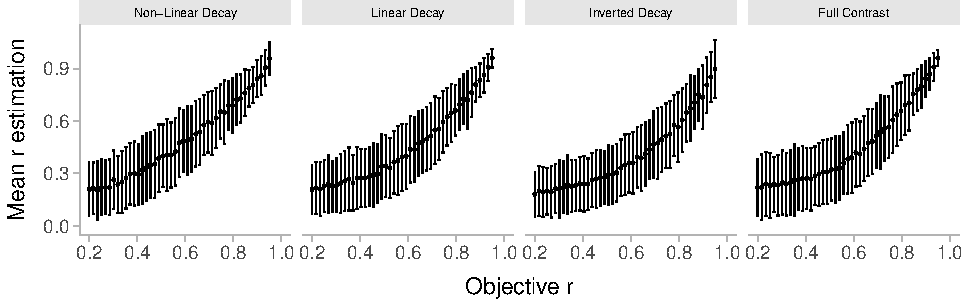
\includegraphics{contrast_and_scatterplots_files/figure-latex/e2-error-plot-1} 

}

\caption{\label{e2-error-plot}The mean of participants' estimations of \textit{r} compared with objective Pearson's \textit{r}, plotted by contrast condition}\label{fig:e2-error-plot}
\end{figure}

Figure \ref{e2-error-plot} shows how participants' mean estimates of
correlation change with the objective Pearson's \emph{r} value, plotted
separately for each of our contrast decay manipulation conditions. We
again observe underestimation curves similar to those reported in
previous literature (see section \ref{testing} and figure
\ref{underestimation-curve}).

\hypertarget{discussion-1}{%
\subsection{Discussion}\label{discussion-1}}

Our hypotheses were fully supported in this experiment. Participants'
errors in correlation estimation were lower when the non-linear decay
parameter was used, and were highest when the non-linear inverted decay
parameter was used. The only surprising result was the lack of
significant difference in correlation estimates between the linear decay
parameter and the full-contrast condition. On closer inspection of the
scatterplots included in the linear decay parameter condition however,
it becomes clear why; the logarithmic nature of contrast perception
\citep{varshney_2013, fechner_1948} means that there is little
perceptual distance between contrasts with high (\textgreater{} 0.75)
contrast alpha values, which translates in our study to no perceived
differences, on average, between plots with linear decay parameters and
full contrast. This apparent threshold for contrast effects was also
found in experiment 1. Filtering out lower \emph{r} values, those with
naturally higher total residuals (arbitrarily \emph{r} \textless{} 0.6),
still produces no significant differences between correlation estimation
errors for linear decay and full contrast conditions (\(\chi^2\)(1) =
0.09, \emph{p} = .769). Our effects sizes were again small in this
experiment, with the largest representing the difference between full
contrast and inverted non-linear decay conditions. This suggests that it
is easier to induce greater bias in correlation estimates through a
reduction in salience of the point clouds centre than it is to correct
for the underestimation bias.

\begin{figure}

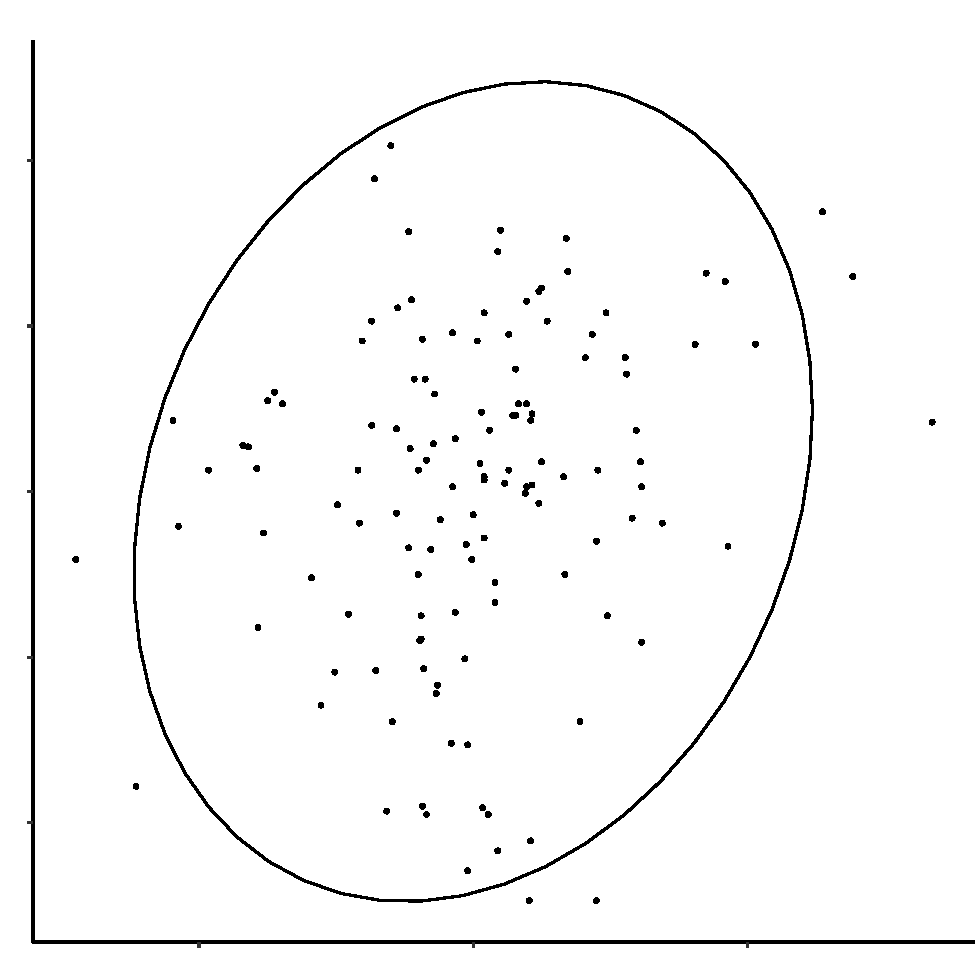
\includegraphics[width=0.5\linewidth]{contrast_and_scatterplots_files/figure-latex/prediction-ellipse-1} \hfill{}

\caption{\label{prediction-ellipse}The above plot shows a 95\% prediction ellipse over a scatterplot with an \textit{r} value of 0.6.}\label{fig:prediction-ellipse}
\end{figure}

Our finding that the use of the non-linear inverted decay parameter, in
which contrast was increased with distance from the regression line,
adds perspective to suggestions \citep{yang_2019} that, among other
visual features, the area of a prediction ellipse
\citep{yang_2019, cleveland_1982}, a region used to predict new
observations assuming a bivariate normal distribution (see Figure
\ref{prediction-ellipse} for an example) was a better predictor of
people's performance on correlation judgement tasks than the objective
\emph{r} value was itself. In our non-linear inverted decay parameter
condition, the area of this prediction ellipse did not change, yet
people's estimates of correlation did. It would appear then that the
apparent density of scatterplot points is also having an effect on
people's perceptions of correlation, at least in our experimental
paradigm. Previous research has found that more dense scatterplot
displays are rated as having higher correlation, although this effect is
weak \citep{lauer_1989, rensink_2014}. To fully explore what is driving
the effect seen in the non-linear inverted decay parameter condition,
further work is needed on what exactly people attend to when completing
correlation perception tasks. Eye-tracking studies would be well suited
for this, but as of yet have only been used for simpler tasks such as
the number of, or distance between points \citep{netzel_2017}.

\hypertarget{general-discussion}{%
\section{General Discussion}\label{general-discussion}}

In this paper we examine the effects of scatterplot point contrast on
perceived correlation. We find that lower total contrast is associated
with greater correlation underestimation error, that the use of the
point contrast manipulation described above can partially correct for
this error, and that inverting the aforementioned manipulation is
associated with greater errors in correlation estimation. We suggest
that these findings could be used to develop novel approaches to
visualizing relationships between data while minimising the error in
perceived correlation. The majority of the studies cited in this paper
have used small samples of participants with experience in data science
and statistics to draw their conclusions, often graduate students in
visualization-heavy fields. We argue that this does not inform the
design of commonly used data visualizations in a naturalistic way. In
comparison, we have recruited from much more representative populations,
and have demonstrated that a simple framework can be used with these
groups to gather high quality data and provide conclusions that can, by
design, be thought of as far more naturalistic than studies that have
taken place in labs with experienced participants.

In agreement with much previous research
\citep{rensink_2010, rensink_2012, rensink_2014, rensink_2017, pollack_1960},
we found that participants were more accurate and more precise when the
\emph{r} value was higher. Figures \ref{e1-changes-plot} and
\ref{e2-changes-plot} plot the objective \emph{r} value against the mean
correlation estimates against Pearson's \emph{r} for experiments 1 and 2
respectively. Standard deviations of estimates are shown as error
bars.These plots illustrate, as in many studies cited, the lower levels
of precision and accuracy for \emph{r} values further from 0 or 1.

\begin{figure}

{\centering 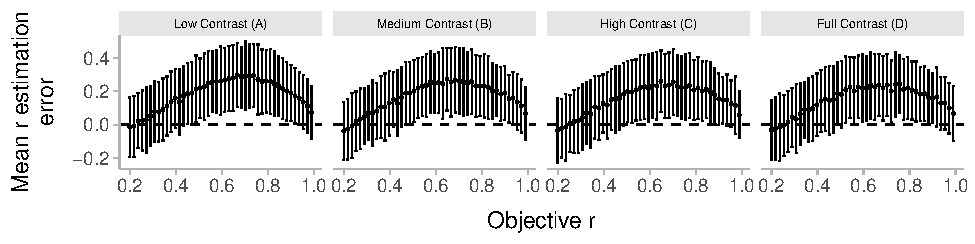
\includegraphics{contrast_and_scatterplots_files/figure-latex/changes-with-r-e1-1} 

}

\caption{\label{e1-changes-plot}Plots showing how participants' mean correlation estimation errors change with Pearson's \textit{r} in experiment 1. Participants were on average most accurate at estimating the \textit{r} value when presented with the full contrast scatterplots (condition D). Error bars show standard deviations of estimates.}\label{fig:changes-with-r-e1}
\end{figure}

\begin{figure}

{\centering 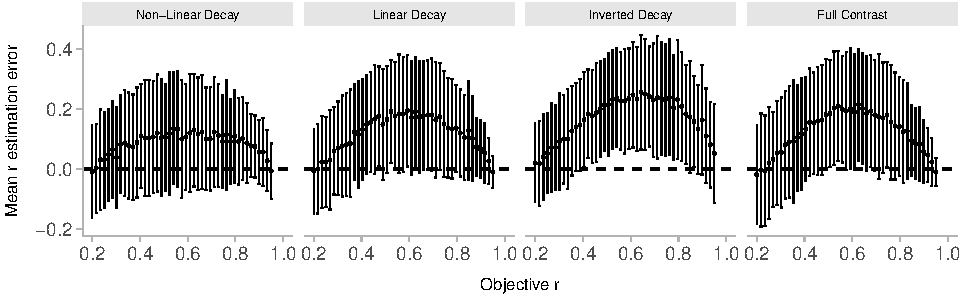
\includegraphics{contrast_and_scatterplots_files/figure-latex/changes-with-r-e2-1} 

}

\caption{\label{e2-changes-plot}Plots showing how participants' mean correlation estimation errors change with Pearson's \textit{r} in experiment 2. Participants were on average most accurate at estimating the \textit{r} value when presented with the non-linear contrast decay scatterplots (condition A). Error bars show standard deviations of estimates.}\label{fig:changes-with-r-e2}
\end{figure}

Our experiments contribute to a body of evidence that suggests
participants are paying attention to the width of the probability
distribution displayed in scatterplots (e.g \citet{cleveland_1982};
\citet{meyer_1997}; \citet{yang_2019}; \citet{rensink_2017}). We also
confirm the systematic underestimation of correlation, and suggest a
strategy to correct for it. Through this work we do not attempt to
redesign the scatterplot as a medium, but to provide a set of
recommendations for visualization designers when designing scatterplots
to support correlation perception:

\begin{enumerate}
\def\labelenumi{\arabic{enumi}.}
\item
  Lowering the total contrast in a scatterplot can cause people to
  underestimate correlation compared to when contrast is maximal between
  the points and the plot background.
\item
  The use of a non-linear contrast decay parameter, in which contrast
  falls as a function of residual size, can be used to counteract the
  underestimation seen in correlation estimation in scatterplots.
\end{enumerate}

Scatterplots, being as widely used as they are, are designed often with
a number of communicative concepts in mind. When one of these concepts
is illustrating to people the degree of association between two
variables, we would argue that designers should utilize the technique we
have described here to give visualization viewers the best chance of
interpreting the correlation displayed as accurately as possible.

\hypertarget{training}{%
\section{Training}\label{training}}

Both experiments described in the current work tested lay participants
with varying levels of graph literacy. Because of this, participants
first saw four plots depicting several correlations (see figure
\ref{example-plots}) to familiarize them with the concept. To test if
the patterns we observed in correlation perception were as a result of
this training, we built a model including the half of the session (first
or second) as a predictor. Comparing this to the original models not
including session half as a predictor revealed a significant effect in
experiment 1 (\(\chi^2\)(1) = 7.13, \emph{p} = 0.01), but not experiment
2 (\(\chi^2\)(1) = 2.20, \emph{p} = 0.14). In experiment 1, participants
errors in correlation estimation were on average higher in the second
half of the experiment, suggesting that having recently viewed correctly
labelled scatterplots helped participants make more accurate judgements
of correlation. That we did not observe this effect in experiment 2
suggests that the influence of our manipulation (the contrast decay
function) had a greater influence on correlation estimation than any
effect of training.

Future work might examine correlation estimation when no training is
offered, or when training is incorrect. Given the quick and intuitive
nature of correlation perception reported in the literature
\citep{rensink_2014}, we would expect only a small effect of training,
although the boundary conditions of such a manipulation are currently
unknown.

\hypertarget{limitations}{%
\section{Limitations}\label{limitations}}

The results in experiment 2 provide evidence that reducing the salience
of points as they move further from the regression line can increase
people's estimates of correlation, at least when plots like these are
presented with other, conventional ones. Testing whether this phenomenon
would exist with a plot in isolation would present a number of
difficulties. As can be seen in figures \ref{e1-dot-plot} and
\ref{e2-dot-plot}, and as more specifically illustrated in Figures
\ref{e1-changes-plot} and \ref{e2-changes-plot}, participants' estimates
of correlation, especially between 0.2 and 0.7, suffer from high
variance. Our high numbers of trials and participants ameliorate this to
an extent, but this does by necessity mean we are unable to comment on
judgements made on single plots.

We have made an important first step in the utilization of contrast
changes to optimize perception of correlation in scatterplots, however
there remains much to do. We were unable to quantitatively determine if
0.25 is indeed the most optimal value for \(b\) in equation 1, for
example. It may well be the case that changing the value of \(b\) as a
function of the objective Pearson's \emph{r} value could produce more
accurate correlation estimates in participants; our finding that
participants were more accurate in correlation estimation when \emph{r}
was nearer 0 or 1 would suggest that the use of a decay parameter for
these correlations is unnecessary.

\hypertarget{future-work}{%
\section{Future Work}\label{future-work}}

In this paper we worked strictly with positive \emph{r} values,
primarily because that is what has been investigated in the majority of
the research that informed ours. However, given previous work
\citep{sher_2017} which found evidence for people overestimating
negative correlation values, it would be reasonable to expect that the
technique we have developed here could also be used to address this bias
also. We predict that the use of our non-linear inverted decay parameter
will reduce the overestimation bias seen in estimates of correlation for
negatively correlated scatterplots.

Our manipulations have used only the vertical distance between a
particular point and the regression line to set contrast. Previous work,
some of which has been inconclusive \citep{meyer_1997}, has generally
suggested that the perpendicular distance between a point and the
regression line may be a more accurate predictor of performance on
correlation estimation tasks
\citep{cleveland_1982, yang_2019, rensink_2017}. Future work
investigating if a difference in correlation estimation accuracy might
be found between contrast decay functions using vertical (residual)
point-line distances or perpendicular ones could further hone the
manipulation.

\hypertarget{acknowledgements}{%
\section{Acknowledgements}\label{acknowledgements}}

This work was supported by funding from the University of Manchester
Department of Computer Science.

\renewcommand\refname{References}
\bibliography{contrast-scatterplots.bib}


\end{document}
